\documentclass[20 pts]{article}
\usepackage{xeCJK}
\usepackage{amsfonts}
\usepackage{amssymb}
\usepackage{amsmath}
\usepackage{bm}
\setCJKmainfont{SimSun}
\title{Review of Deterministic Interleavers}
\author{Kwame Ackah Bohulu}
\date{25-05-2017}
\begin{document}
\maketitle


\section{Introduction}
 ターボ符号が発見された年から、符号の良い性能を詳しく理解するため、たくさんの研究がされている。研究で当然になったことは、ターボ符号器のインタリーバがターボ符号の性能に影響を与える。インタリーバの働きは、低い重みを持つターボ符号の符号語の数を減る(へる)ことである
[1]。長いフレームサイズの場合、インタリーブとデインタリーブがアルゴリズムでできるので、決定論インタリーバ がよく使われている[3]。ターボ符号が高いエラーフローを持ち、固定されたインタリーバの長さ$N$で、エラーフローを減るのに、ターボ符号の自由距離の値を大きくしながら、自由距離の重みをもつ符号語の数を維持(いじ)する[1]。この資料で、基本の決定論インタリーバを復習し、インタリーバの距離性質を増やす方法を説明する。

\section{ブロックインタリーバと線形インタリーバ}
基本の決定論インタリーバはブロックインタリーバと線形インタリーバである[3]。ブロックインタリーバは、$N=m\times n$の大きさの方形行列(ほうけいぎょうれつ)で定義されている。  入力ビットの位置は、行ごとに書き、インタリーバするときは、列ごとによむ。ブロックインタリーバのマッピング関数は(1)で定義されている[2]。

$$\Pi_{\mathfrak{B}_N} \equiv ni + \lfloor l/m\rfloor \mod {N},		0\leq i < N.$$
線形インタリーバのマッピング関数は(2)で定義されている。

$$\Pi_{\mathfrak{L}_N} \equiv ki + v \mod {N},		0\leq i < N.$$
$k$は、$N$と互いにそう固定された整数であり、$v$は固定された整数である。

 線形インタリーバは、(2)の$\lfloor \dot \rfloor$部分を線形化することがわかる。
ブロックインタリーバと線形インタリーバは線形合同(せんけいごうどう)に基づいているので、それぞれの性質がかなり近いです。

例えば、ブロックインタリーバの場合、定数$t\mod {N}$ で離れる入力系列の二位置は、定数$tn\mod{n}$で離れる出力系列に対する二位置にマップし、線形インタリーバの場合、定数$tk
\mod{n}$で離れる出力系列に対する二位置にマップする。

定数 $k$ は線形インタリーバの角係数と呼ばれ、ブロックインタリーバの角係数はインタリーバの長さと等しいである[2]。ブロックインタリーバは線形インタリーバの性質と等しいため、ブロックインタリーバの分析は線形インタリーバを使用する。

角係数はインタリーバの性能に影響を与える。  重み2を持つ入力系列がターボ符号の自由距離に影響を与える。線形インタリーバは悪い重み2を持つ入力系列に弱いである。悪い入力系列とは、低い重みをもつターボ符号の符号語を出す系列である。 悪い入力系列を良い入力系列
にするために以下で説明された角係数を選択する方法を使用すればよいである。

 入力系列の位置$x_a$と$x_b$と出力系列と同じ位置$y_a$と$y_b$の間の距離の和の最低値に$\sqrt{2N}$にするため、、角係数の値を $\sqrt{2N}$に近い整数値にしたらよいである[4]。しかし、[2]でわかることは、角係数の値を$\sqrt{N}$ にしたら、それぞれの位置の間の距離の和の最低は大きく、ターボ符号の自由距離を大きくするので、$\sqrt{N}$は角係数の十分値である。
 
また、xからyまでマッピングされた位置の間の距離が要素符号のcycle length $\tau$の倍数にならないように注意する必要がある。そうならないように、シムレーションで、$\tau$の倍数距離でのすべての重み2を持つ入力系列に対するターボ符号の符号語の重みを計算し、$\sqrt{N}$のオーダーまでの角係数を使用し、ターボ符号のBER $P_b(e)$を計算する。
BER $P_b(e)$は (3)で計算できる。



\begin{equation}
P_b \approx \frac{1}{2}\sum_{w_c}D_{w_c}erfc\Big (\, \sqrt{w_c \frac{R_cE_b}{N_o}} \Big)\,
\end{equation}
where
\begin{equation*}
D_{w_c} \triangleq \sum_{w_i+w_p=w_c}\frac{w_i}{N}A_{w_i,w_p}
\end{equation*}

$w_i$ は、入力系列の重みであり、$w_p$ はパリティ系列の重みであり、$A_{w_i,w_p}$は$w_i$と$w_p$ を持つターボ符号の符号語の数である。

ある2つの線形インタリーバの図とランダムインタリーバの図はfig. 1 と fig. 2 で描かれている

\begin{figure}[!]
\centering
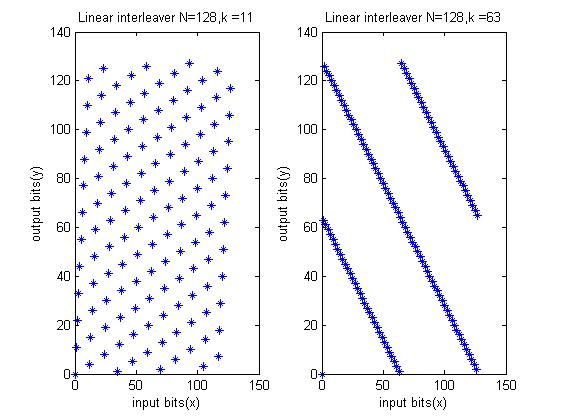
\includegraphics[width=0.5\textwidth,]{zemi2fig3.jpg}
\caption{Graphical representation of Linear interleaver with N=128, v=0 and k =[11,63]}
\label{}
\end{figure}

\begin{figure}[!]
\centering
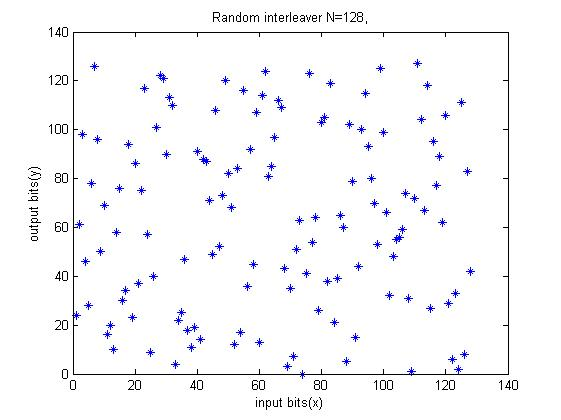
\includegraphics[width=0.5\textwidth,keepaspectratio]{zemi2fig4.jpg}
\caption{Graphical representation of Random interleaver with N=128}
\label{}
\end{figure}




\newpage
\section{References}
\paragraph{[1]}  Oscar Y. Takeshita, Member, IEEE, and Daniel J. Costello ,''New Deterministic Interleaver Designs for Turbo Codes'',IEEE Trans. Inform. Theory, vol.  46,pp. 1988-2006,Nov. 2000\\
\paragraph{[2]}  L. C. Perez, J. Seghers, D. J. Costello, Jr., ''A distance spectrum interpretation of turbo codes'', IEEE Trans. Inform. Theory, vol. 42, pp. 1698-1709, Nov. 1996.\\
\paragraph{[3]} Jing Sun, Oscar Y. Takeshita ”Interleavers for Turbo Codes Using Permutation Polynomials over Integer Rings”, IEEE Trans. Inform. Theory, vol. 51,
pp. 101 - 119 Jan. 2005\\
\paragraph{[4]}S. Dolinar and D. Divsalar, “Weight distribution of turbo codes using
random and nonrandom permutations,” JPL, TDA Progr. Rep. 42-122,
Aug. 1995.



\end{document}